\subsubsection*{Оценка моделей по критериям}

\begin{center}
    Таблица 2. Оценка всех моделей проекта в соответствии с заявленными критериями
\end{center}

\begin{center}
    \textbf{Модель №1}
\end{center}

\begin{longtable}{|l|l|l|}
    \hline
    \multicolumn{3}{|c|}{\textbf{Оригинальное здание} } \\
    \hline
    \multicolumn{3}{|c|}{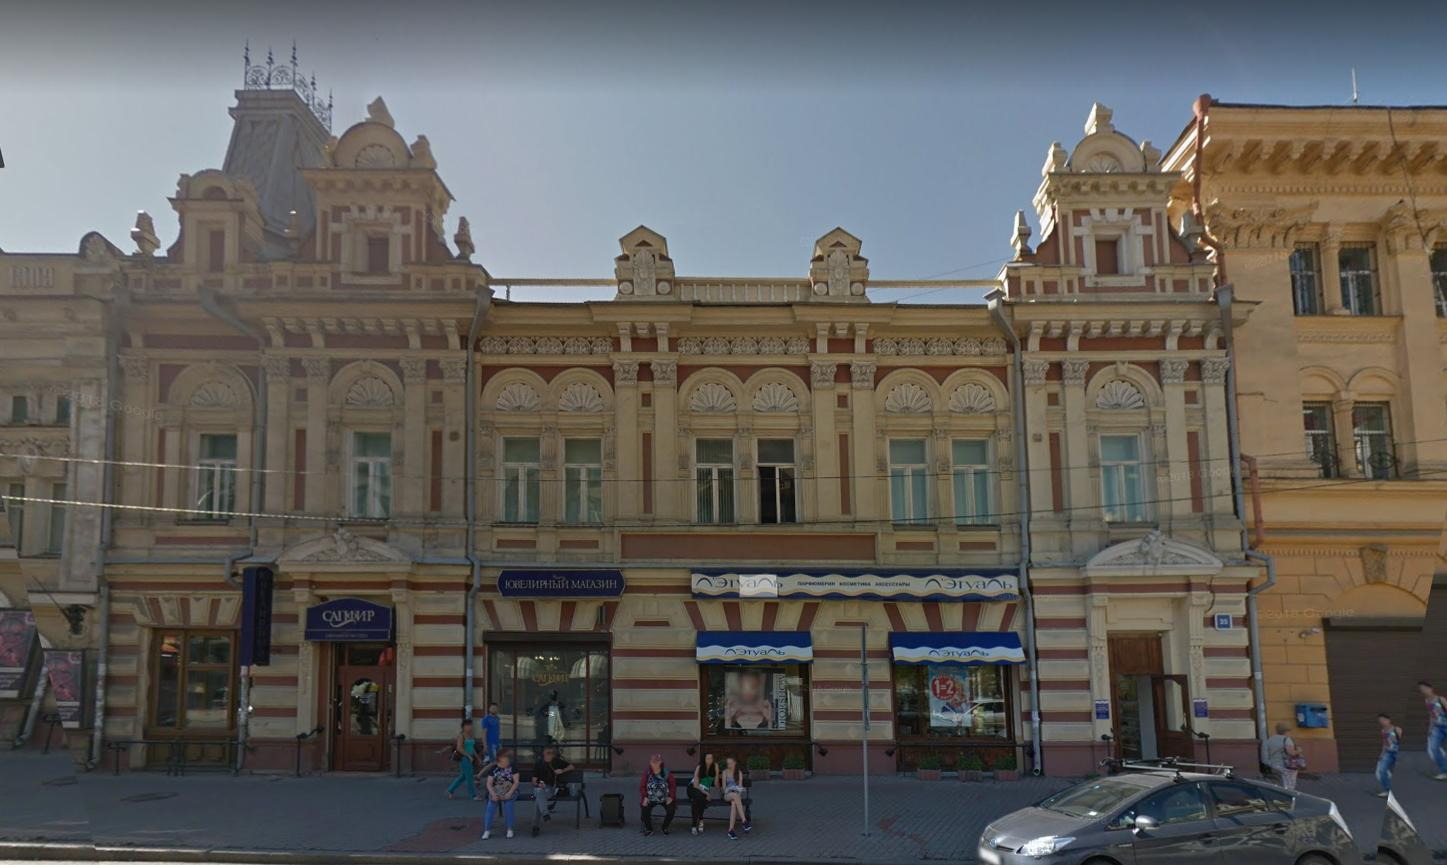
\includegraphics[width=7cm]{1}} \\
    \hline
    \multicolumn{3}{|c|}{\textbf{Модель}} \\
    \hline
    \multicolumn{3}{|c|}{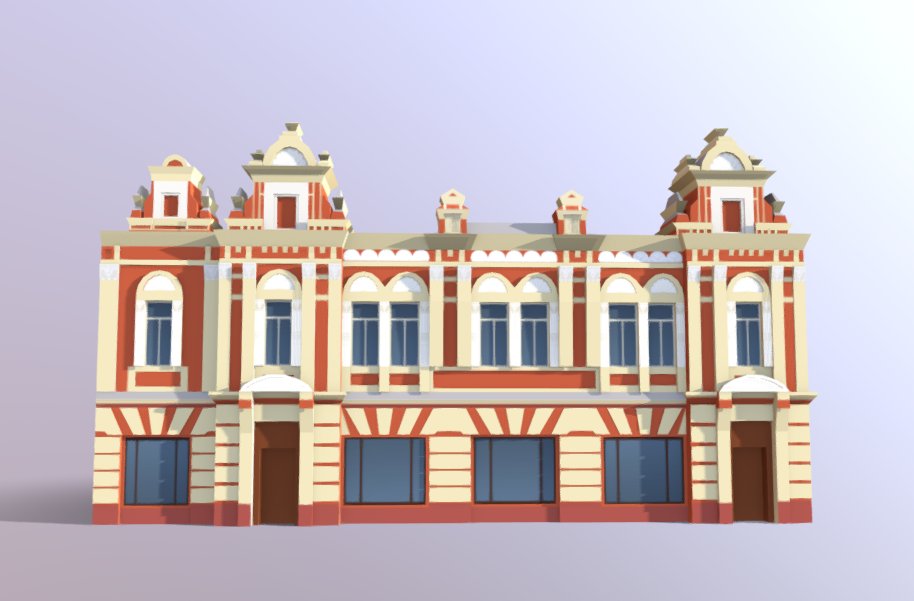
\includegraphics[width=7cm]{model_1}} \\
    \hline
    \textbf{Критерий} & \textbf{Балл/Max.балл} & \textbf{Комментарии} \\
    \hline
    Количество полигонов < 3k. & 0.9/0.9 & Количество полигонов - 2 695, соответствует допустимому диапазону. \\
    \hline
    Детализация. & 0.7/0.7 & Модель не является примитивом, отдельные части не перегружены лишними деталями, детализация не влияет на критерий количества полигонов. \\
    \hline
    Сходство с реальным объектом. & 0.7/0.7 & Объект можно легко опознать при сравнении с оригиналом - сохранены общие пропорции здания, характерные детали и количественный фактор (окна, двери и т.п.) \\
    \hline
    UV-развертка. & 0.6/0.6 & Развертка присутствует. Вес развертки правильный (окрашена в равномерный синий цвет без ярких зеленых или желтых зон).

    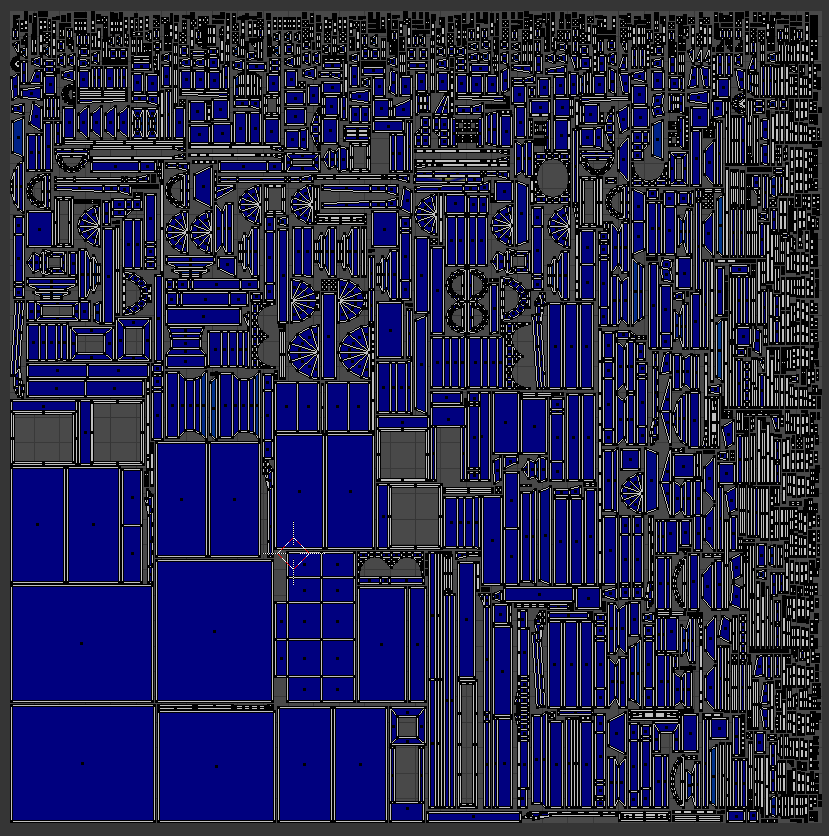
\includegraphics[width=7cm]{uv_1} \\
    \hline
    Наличие текстур. & 2.0/2.0 & Текстура присутствует (+ дополнительная текстура для ambient occlusion), все текстурные элементы запечены на одну текстуру.

    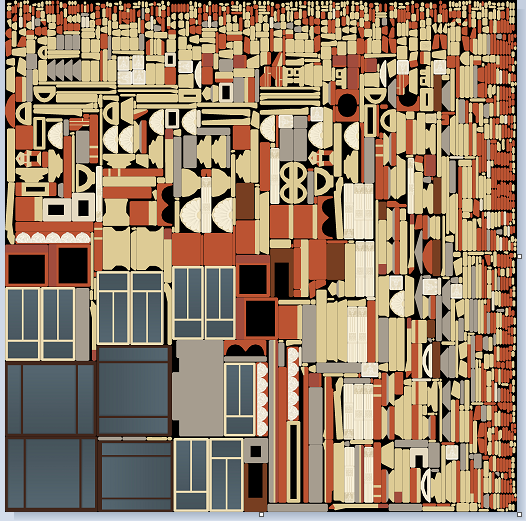
\includegraphics[width=7cm]{tec_1}

    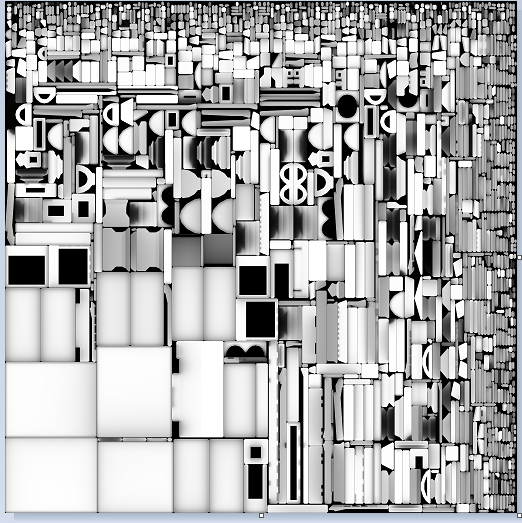
\includegraphics[width=7cm]{tec_2}\\
    \hline
    Отсутствие перевернутых нормалей. & 0.45/0.45 & Оси нормалей отображаются верно, направлены из объекта, а не вовнутрь. Нет затемненных участков меша или участков объекта без отображаемых текстур (свидетельство перевернутых нормалей).

    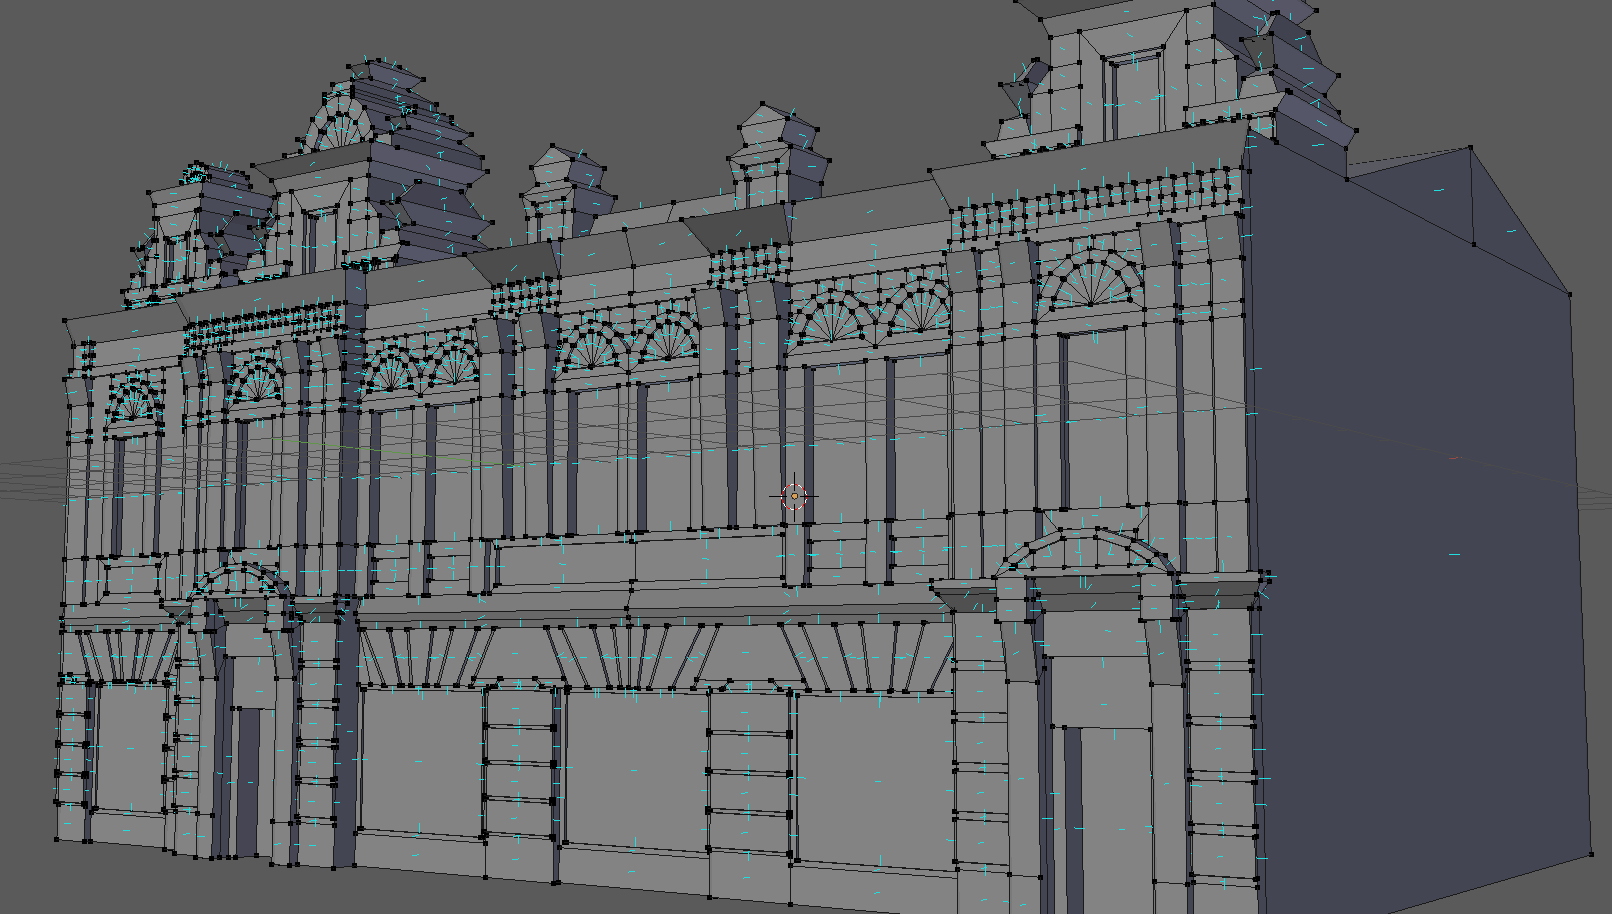
\includegraphics[width=7cm]{norm_1}

    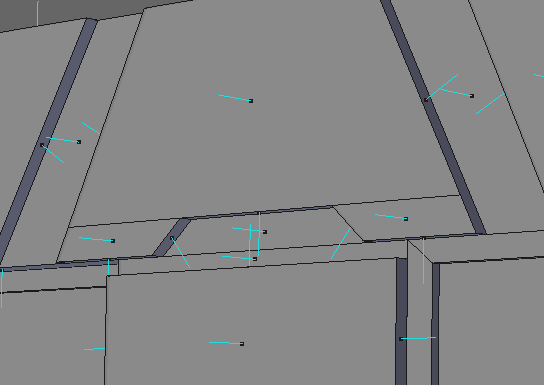
\includegraphics[width=7cm]{norm_2}\\
    Отсутствие неправильных полигонов. & 0.6/0.6 & Все полигоны имеют форму четырехугольника или треугольника, нет полигонов с бо́льшим количеством углов. \\
    \hline
    \multicolumn{3}{|c|}{\textbf{Итого за модель: 5.95}} \\
    \hline
\end{longtable}

\begin{center}
    \textbf{Модель №2}
\end{center}

\begin{longtable}{|l|l|l|}
    \hline
    \multicolumn{3}{|c|}{\textbf{Оригинальное здание} } \\
    \hline
    \multicolumn{3}{|c|}{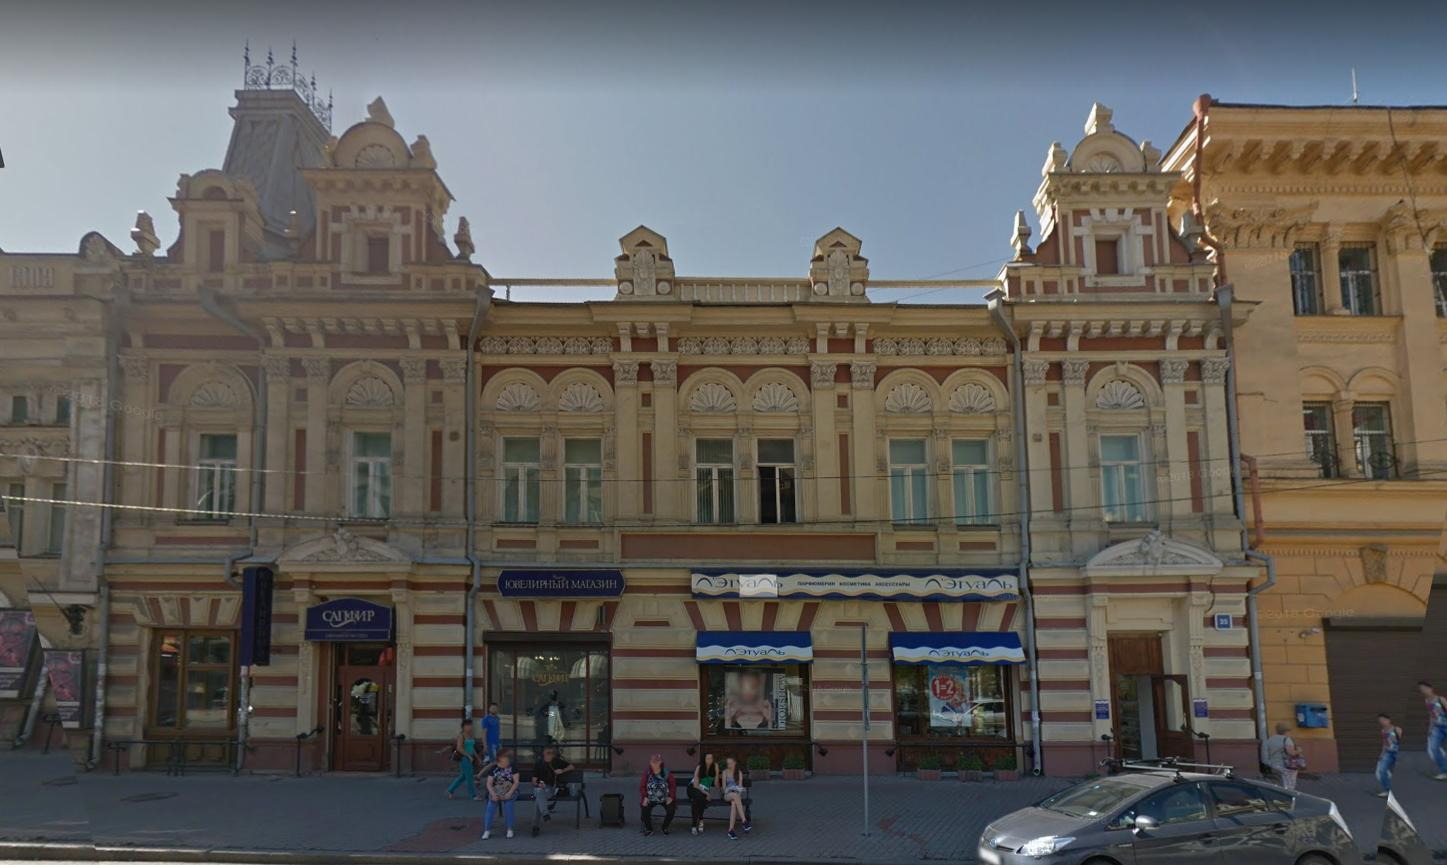
\includegraphics[width=7cm]{1}} \\
    \hline
    \multicolumn{3}{|c|}{\textbf{Модель}} \\
    \hline
    \multicolumn{3}{|c|}{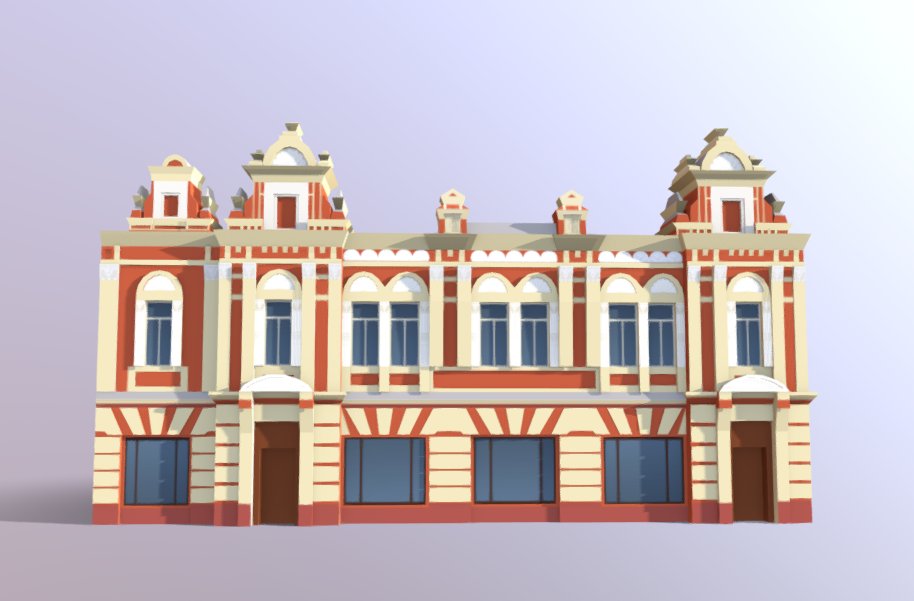
\includegraphics[width=7cm]{model_1}} \\
    \hline
\end{longtable}